\section{Zpětnovazebné učení}

% ----------------------------------------------------------------------------

\section{Modely, co se učí samy}


\begin{frame}{Modely, co se učí samy}

    \begin{itemize}[<+->]

        \item Většina, co jsme viděli, trénované z~párů \emph{vstup-výstup}
            \\ \quad\emph{supervised learning} (učení s~učitelem)

        \item Modely se mohou učit od sebe navzájem

        \item Reinforcement learning -- AlphaGo: Model hraje Go s~různými
            verzemi sebe sama \\ {\tiny \citep{singh2017learning}}

        \item Zpětný překlad ve strojovém překladu: překlad jednojazyčných
            textů je vstup do překladače na druhou stranu {\tiny \citep{sennrich2016improving}}

        \item Generativní adversariální sítě\ldots

    \end{itemize}

\end{frame}

% ----------------------------------------------------------------------------


\begin{frame}{Generator-discrimitor}

    \begin{itemize}[<+->]

        \item Většina, co jsme viděli, trénované z~párů \emph{vstup-výstup}

        \item Hrají proti sobě dvě neuronové sítě: {\bf generátor} a {\bf
            diskriminátor}

    \end{itemize}

    \vspace{10pt}

    \begin{columns}[t]
        \column{.45\textwidth}
        \visible<3->{\textbf{Generátor}}

        \begin{itemize}

            \item<4-> Má v~sobě prvek náhody: umožňuje generovat rozmanité výstupy

            \item<5-> Snaží se vyprodukovat takový výstup, aby
                \textbf{diskriminátor nepoznal}, jestli, že jde o generovaný
                příklad

        \end{itemize}

        \column{.45\textwidth}
        \visible<6->{\textbf{Diskriminátor}}

        \begin{itemize}

            \item<6-> Pracuje s~reálnými data a generovanými daty

            \item<7-> Snaží se naučit \textbf{rozpoznat syntetická a autentická
                data}


        \end{itemize}

    \end{columns}

    \vspace{10pt}

    \tiny Koncept GAN poprvé představil \citet{goodfellow2014generative}

\end{frame}

% ----------------------------------------------------------------------------

\begin{frame}{This person does not exist}

    \centering
    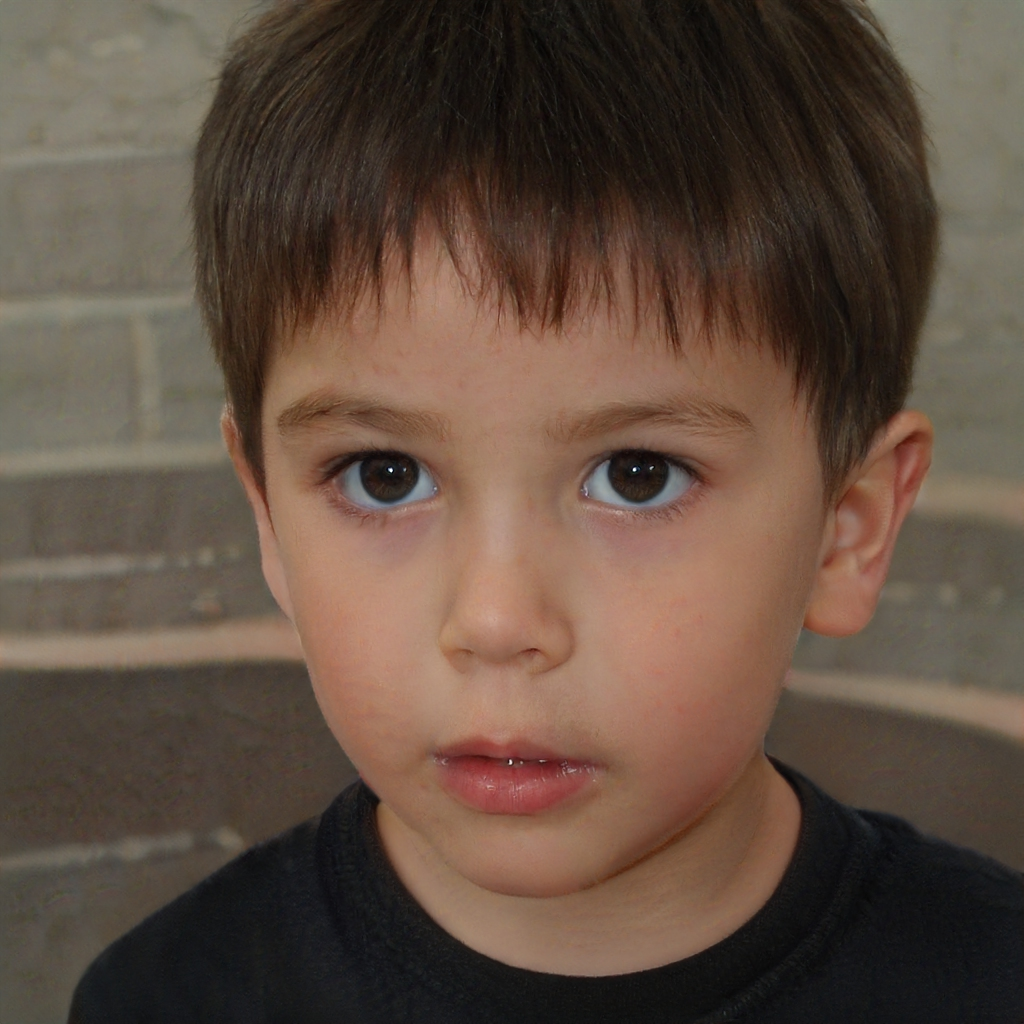
\includegraphics[width=65pt]{img/person1.jpeg}
    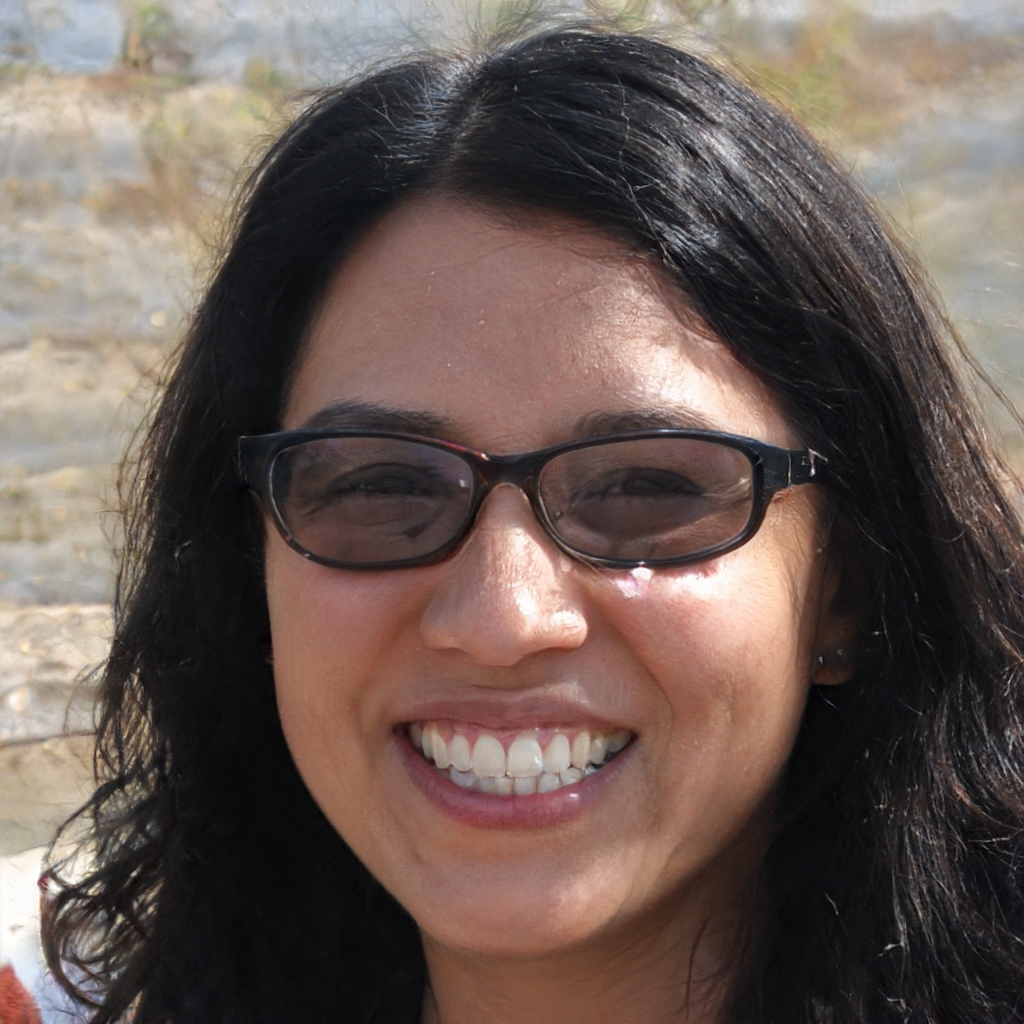
\includegraphics[width=65pt]{img/person2.jpeg}
    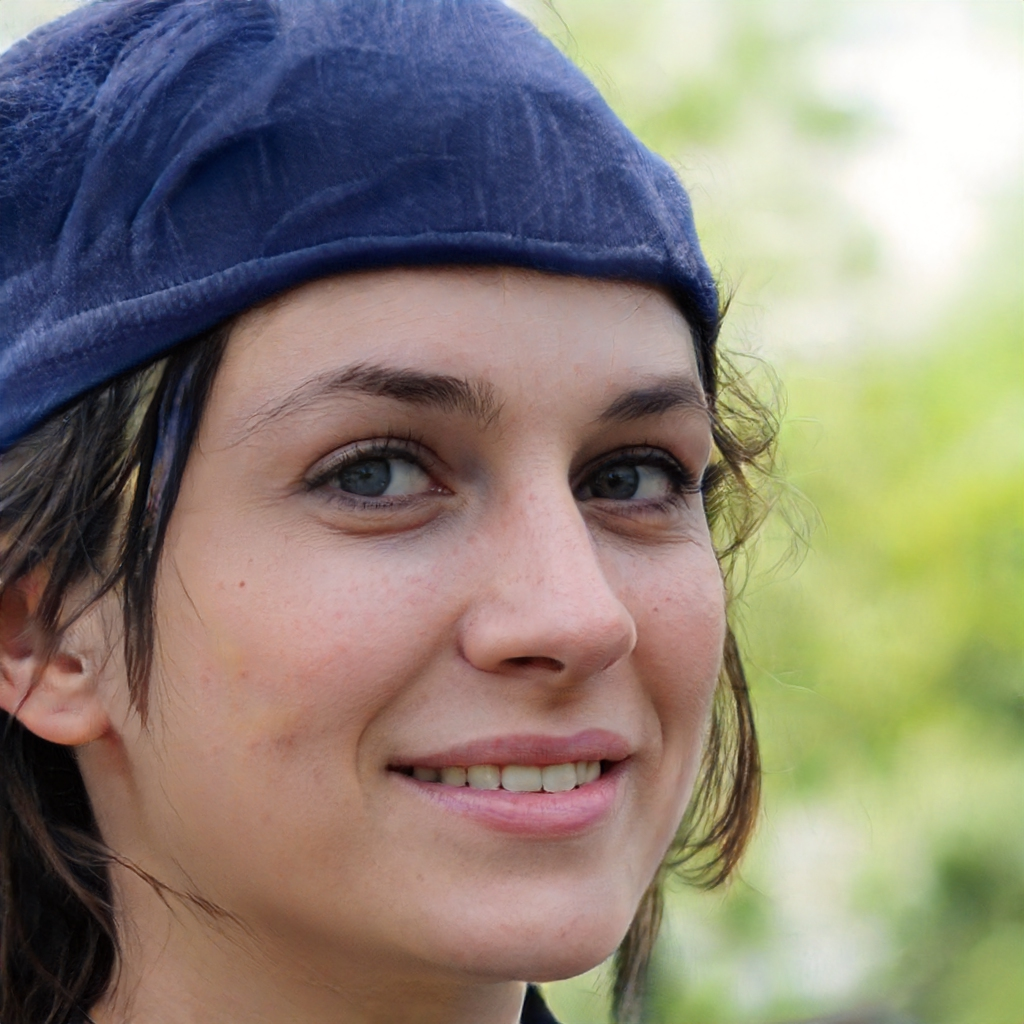
\includegraphics[width=65pt]{img/person3.jpeg}
    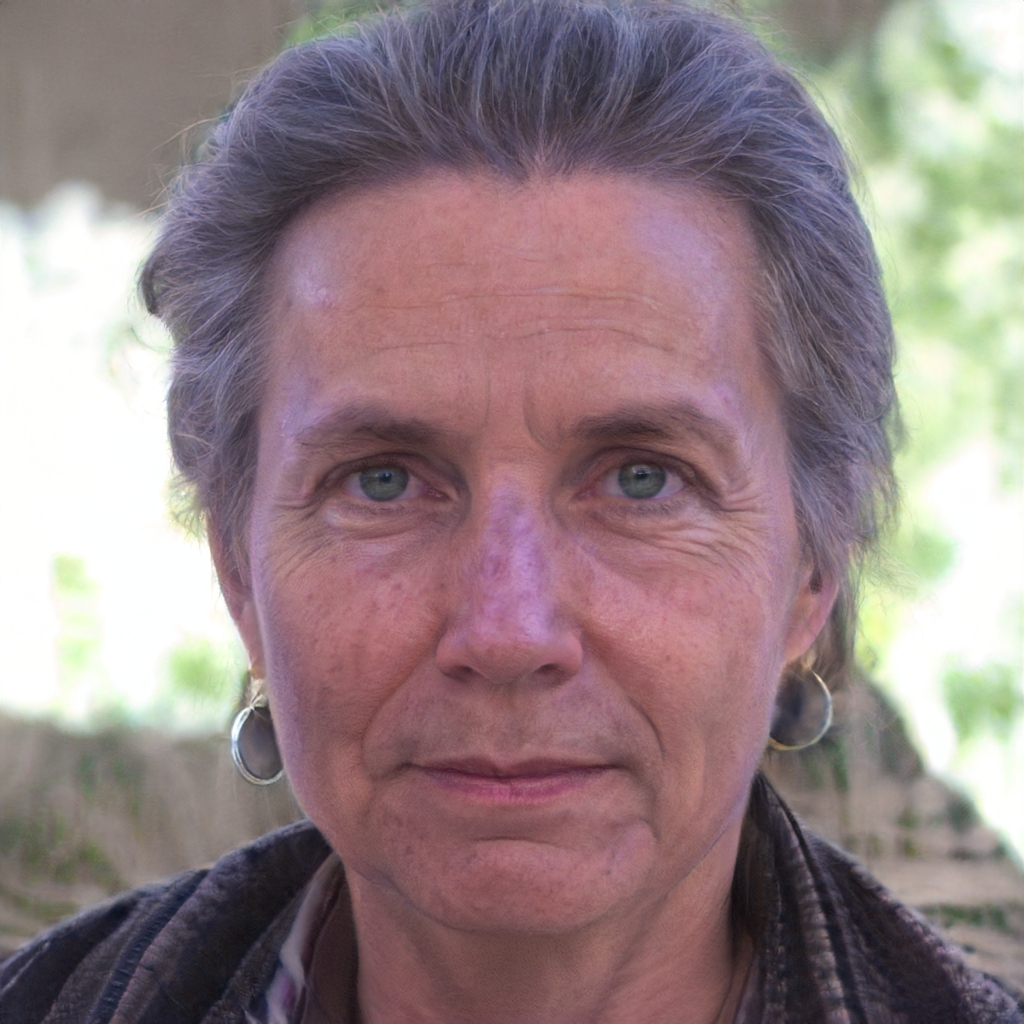
\includegraphics[width=65pt]{img/person4.jpeg} \\
    {\tiny Vygenerováno s~pomocí \url{https://thispersondoesnotexist.com/},
    model z~článku \citet{karras2020analyzing}}

    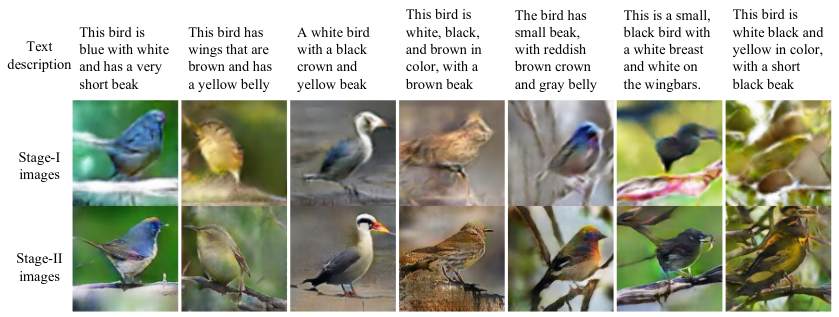
\includegraphics[scale=.35]{img/gan_birds.png} \\
    {\tiny Zdroj \citet[obr.\ 5]{zhang2017stack}}

\end{frame}

% ----------------------------------------------------------------------------

\begin{frame}{Deepfakes}

    \begin{center}

        {\Large = falešná videa, kam se dosadí tvář jiného člověka} \\

        (pornografie, politická propaganda)

    \end{center}

    \vspace{15pt}

    \visible<2->{Generátor optimalizuje pro dva cíle:}

    \begin{enumerate}

        \item<3-> Model, který rozpoznává obličeje, musí rozpoznat správnou osobu

        \item<4-> Diskriminátor nesmí poznat, co že je to fake

    \end{enumerate}

\end{frame}

 ----------------------------------------------------------------------------

\begin{frame}{Co se nevešlo \ldots}

    \begin{itemize}

        \item Difusion modely pro generování obrázků (DALLE-2)

        \item AlphaFold: predikce strutury proteinů

    \end{itemize}

\end{frame}